
% Mention more about Fortran types
%
% Make a conclusion statement

\documentclass{beamer}

\usepackage{fontspec}
\usepackage{physics}
\usepackage{minted}
\usepackage{color}
\usepackage{amsfonts}
\usepackage{amsmath}
\usepackage{xcolor}
\usepackage{mathrsfs}
\usepackage{mathtools}
\usepackage{forest}

\usepackage[backend=bibtex, style=verbose-trad2]{biblatex}
\bibliography{automated-unit-checking-in-neuron-simulations}{}

\newcommand{\overbar}[1]{\mkern 1.5mu\overline{\mkern-1.5mu#1\mkern-1.5mu}\mkern 1.5mu}

\makeatletter
\def\blfootnote{\xdef\@thefnmark{}\@footnotetext}
\makeatother

\title{Automated Unit Checking In Neuron Simulations}
\author{Scott Urnikis (Dr. E. Rosa)}

\begin{document}
\maketitle

%%%%%%%%%%%%%%%%%%%%%%%%%%%%%%%%%%%%%%%%%%%%%%%%%%%%%%%%%%%%%%%%%%%%%%%%%%%%%%%%
%                                                                              %
%            Introduce the first simulation: hodgkin-huxley                    %
%                                                                              %
%%%%%%%%%%%%%%%%%%%%%%%%%%%%%%%%%%%%%%%%%%%%%%%%%%%%%%%%%%%%%%%%%%%%%%%%%%%%%%%%

\begin{frame}[fragile]

  The Hodgkin Huxley Equations are a set of coupled first order differential equations
  that model the flow of electric current over the surface membrane of a large nerve fiber.

  \vspace{2mm}

  \begin{align*}
    C\dot{\text{V}} & = I
    - \overbar{g_{K}}\text{n}^{4}(V - E_{K})
    - \overbar{g_{Na}}\text{m}^{3}\text{h}(V - E_{Na})
    - g_{L}(V - E_{L}) \\
  \end{align*}
  
  \begin{align*}
    \dot{\text{n}} & = 0.01\frac{10 - V}{e^{10-\frac{V}{10}}}(1 - \text{n}) - 0.125 \text{n} e^{\frac{-V}{80}} \\
    \dot{\text{m}} & = 0.1\frac{25 - V}{e^{25 - \frac{V}{10}} - 1}(1 - \text{m}) - 4 \text{m} e^{\frac{-V}{18}} \\
    \dot{\text{h}} & = 0.07 e^{\frac{-V}{20}}(1 - \text{h}) - \frac{\text{h}}{e^{3 - \frac{V}{10}} + 1}
  \end{align*}

  \blfootnote{J Physiol. Hodgkin and Huxley. 1952}
\end{frame}

%\begin{frame}[fragile]
%  \begin{minted}{C++}
%    double const I      10.0  // micro A
%    double const C      1.0   // micro F / cm^2
%    double const g_Na   120.0 // mS / cm^2
%    double const g_K    36.0  // mS / cm^2
%    double const g_L    0.3   // mS / cm^2
%    double const E_Na   120.0 // mV 
%    double const E_K   -12.0  // mV
%    double const E_L    10.6  // mV 
%  \end{minted}
%\end{frame}

% \begin{frame}[fragile]
%  \begin{minted}{C++}
%    // A neuron with initial conditions
%    // for V, n, m, and 
%    
%    Neuron example_neuron {
%      65.0, // mV
%      0.0,  // none
%      0.0,  // none
%      0.0   // none
%    }; 
%  \end{minted}
%\end{frame}

{
  \setbeamertemplate{navigation symbols}{}
  \setbeamertemplate{background canvas}{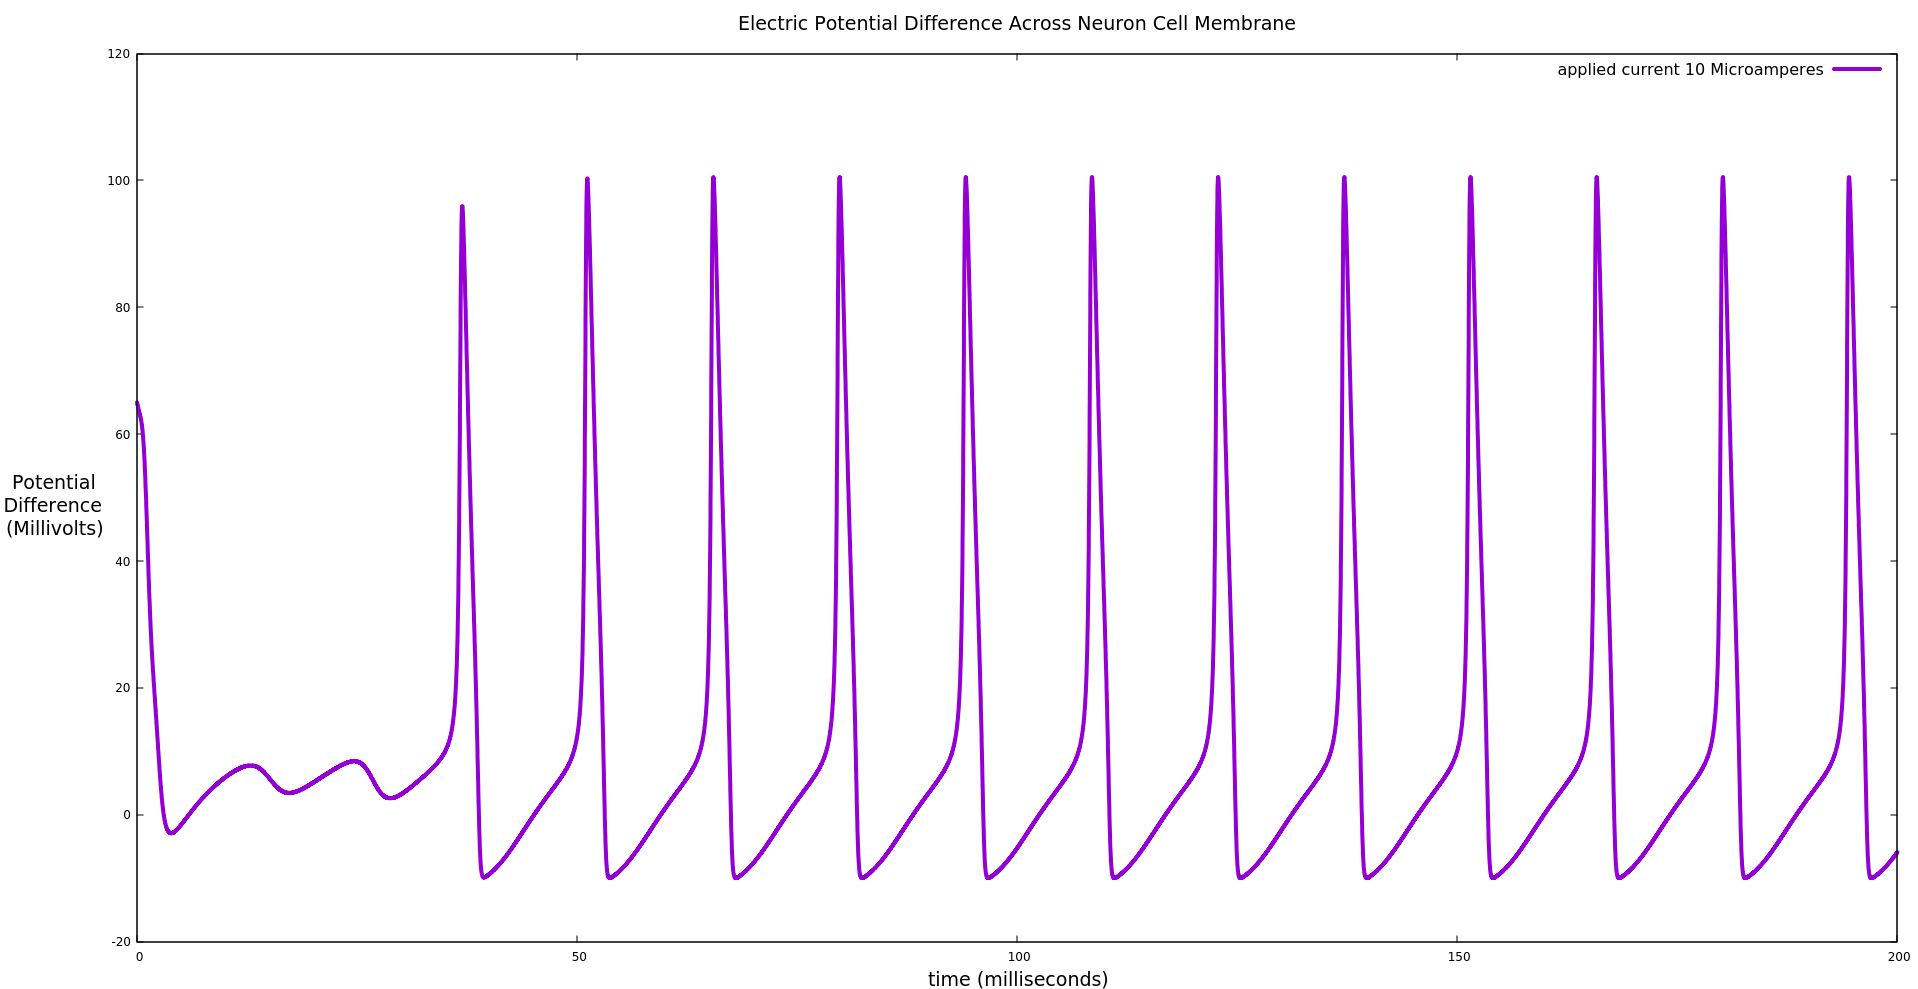
\includegraphics[height = \paperheight, 
      width = \paperwidth]{10MicroampereHH.png}}
  \begin{frame}[plain]
  \end{frame}
}

\begin{frame}[fragile]
  \begin{minted}{C++} 
    return (I - g_K*pow(n, 4)*(V - E_K)
       - g_Na*pow(m, 3)*h*(V - E_Na)
       - g_L*(V - E_L))
       / C;
  \end{minted}
\end{frame}

\begin{frame}[fragile]
  \begin{equation*}
    \frac{I - g_k \cdot n^4 \cdot \left(V - E_K\right) - g_{Na} \cdot m^3 \cdot h \cdot (V - E_{Na}) - g_L \cdot
      \left(V - E_L\right)}
         {C}
  \end{equation*}
\end{frame}

\begin{frame}[fragile]
  \begin{equation*}
    \frac{\text{d} - \text{d} \cdot \text{d}^4 \cdot \left(\text{d} - \text{d}\right) - \text{d} \cdot \text{d}^3 \cdot \text{d} \cdot (\text{d} - \text{d}) - \text{d} \cdot \left(\text{d} - \text{d}\right)}
         {\text{d}}
  \end{equation*}
\end{frame}

\begin{frame}[fragile]
  \begin{equation*}
    \frac{\text{d} - \text{d} \cdot \text{d}^4 \cdot \text{d} - \text{d} \cdot \text{d}^3 \cdot \text{d} \cdot \text{d} - \text{d} \cdot \text{d}}
         {\text{d}}
  \end{equation*}
\end{frame}

\begin{frame}[fragile]
  \begin{equation*}
    \frac{\text{d} - \text{d} \cdot \text{d} \cdot \text{d} - \text{d} \cdot \text{d} \cdot \text{d} \cdot \text{d} - \text{d} \cdot \text{d}}
         {\text{d}}
  \end{equation*}
\end{frame}

\begin{frame}[fragile]
  \begin{equation*}
    \frac{\text{d} - \text{d} - \text{d} - \text{d}}
         {\text{d}}
  \end{equation*}
\end{frame}

\begin{frame}[fragile]
  \begin{equation*}
    \frac{\text{d}}
         {\text{d}}
  \end{equation*}
\end{frame}

\begin{frame}[fragile]
  \begin{equation*}
    \text{d}
  \end{equation*}
\end{frame}

\begin{frame}[fragile]
  Our hypothesis is that if the user is able to express more information about the
  physics of the simulation, the amount of syntactically correct but semantically incorrect programs can be reduced.
\end{frame}

%%%%%%%%%%%%%%%%%%%%%%%%%%%%%%%%%%%%%%%%%%%%%%%%%%%%%%%%%%%%%%%%%%%%%%%%%%%%%%%%
%                                                                              %
%                 Discuss the Curry-Howard Isomorphism                         %
%                                                                              %
%%%%%%%%%%%%%%%%%%%%%%%%%%%%%%%%%%%%%%%%%%%%%%%%%%%%%%%%%%%%%%%%%%%%%%%%%%%%%%%%

\begin{frame}[fragile]
  We are familiar with the idea of types in programming languages. 
  For example, we might declare that we are going to use a variable \textbf{foo}, where
  \textbf{foo} is of type \textbf{integer}.
  \vspace{4mm}

  In Fortran...
  \begin{minted}{Fortran}
    ! ''foo'' is of type ''integer''
    integer foo
  \end{minted}

  In C{}\verb!++!...
   \begin{minted}{C++}
    // ''foo'' is of type ''int''
    int foo;
   \end{minted}

   \pause
   Using mathematical notation...
   \begin{equation*}
     foo : MachineInt
   \end{equation*}

  \vspace{4mm}
  \pause
  \begin{equation*}
    \{ \text{i} \in \mathbb{Z} \mid -2^{32} <= i <= 2^{32} - 1 \}
  \end{equation*}
\end{frame}

%%%%%%%%%%%%%%%%%%%%%%%%%%%%%%%%%%%%%%%%%%%%%%%%%%%%%%%%%%%%%%%%%%%%%%%%%%%%%%%%
%                                                                              %
%          Describe the implementation of the unit checking system             %
%                                                                              %
%%%%%%%%%%%%%%%%%%%%%%%%%%%%%%%%%%%%%%%%%%%%%%%%%%%%%%%%%%%%%%%%%%%%%%%%%%%%%%%%

\begin{frame}[fragile]
  Could we use types to verify unit cancellation?

  \pause
  \vspace{4mm}
  SI units can be implemented with only seven base units: \pause
  \begin{itemize}
  \item{Distance: meter}
  \item{Mass: kilogram}
  \item{Time: second}
  \item{Temperature: Kelvin}
  \item{Electric current: Ampere}
  \item{Amount of substance: mole}
  \item{Luminous intensity: Candela}
  \end{itemize}
\end{frame}

%\begin{frame}[fragile]
%  The main idea we will be expressing is the idea of a \emph{quantity}.
%
%  \vspace{4mm}
%  
%  A quantity is a numeric value with its unit information included.
%\end{frame}

\begin{frame}[fragile]
  There are many different kinds of quantities, because there are many different units.
  Therefore, what we need is the ability to express a \emph{family} of types, not just a
  single type.

  \vspace{4mm}
  
  For this, we can use a concept from type theory called \emph{dependent types}.
\end{frame}

\begin{frame}[fragile]
  A dependent type is a type that depends on some values. In other words, it is a function that,
  given some parameters, returns a type.

  \begin{equation*}
    Quantity : \mathbb{Z}^7 \to \mathscr{U}
  \end{equation*}

  \pause

  Let $m$, $kg$, $s$, $K$, $A$, $mol$, and $cd$ be integers. Then, a unit can be represented by the type 
  \begin{equation*}
    Quantity\left( \begin{bmatrix*} m \\ kg \\ s \\ K \\ A \\ mol \\ cd \end{bmatrix*} \right)
  \end{equation*}
  where $m$, $kg$, $s$, $K$, $A$, $mol$, and $cd$ represent the exponent of the unit.

  \blfootnote{Homotopy Type Theory. The Univalent Foundations Program. 2013}
  \blfootnote{Scientific and Engineering C++. Barton and Nackman. 1994}
\end{frame}

\begin{frame}[fragile]
  The meter type
  \begin{align*}
    \left[ meter \right] & \\
    meter & \equiv Quantity \left( \begin{bmatrix*} m = 1 \\ kg = 0 \\ s = 0 \\ K = 0 \\ A = 0 \\ mol = 0 \\ cd = 0\end{bmatrix*} \right)
  \end{align*}
\end{frame}

\begin{frame}[fragile]
  The Newton type
  \begin{align*}
    \left[ Newton \right] & = \left[ \frac{kg \cdot m}{s^2} \right] \\
    Newton & \equiv Quantity\left( \begin{bmatrix*}[c] m = 1 \\ kg = 1 \\ s = -2 \\ K = 0 \\ A = 0 \\ mol = 0 \\ cd = 0 \end{bmatrix*} \right) 
  \end{align*}
\end{frame}

\begin{frame}[fragile]
  The Volt type
  \begin{align*}
    \left[ Volt \right] & = \left[ \frac{kg \cdot m^2}{s^3 \cdot A} \right] \\
    Volt & \equiv Quantity\left( \begin{bmatrix*}[c] m = 2 \\ kg = 1 \\ s = -3 \\ K = 0 \\ A = -1 \\ mol = 0 \\ cd = 0\end{bmatrix*} \right) 
  \end{align*}
\end{frame}

% \begin{frame}[fragile]
%  The Farad type
%  \begin{align*}
%    \left[ Farad \right] & = \left[ \frac{s^4 \cdot A^2}{m^2 \cdot kg} \right] \\
%    Farad & \equiv Quantity\left( \begin{bmatrix*}[c] m = -2 \\ kg = -1 \\ s = 4 \\ K = 0 \\ A = 2 \\ mol = 0 \\ cd = 0\end{bmatrix*} \right) 
%  \end{align*}
%\end{frame}

\begin{frame}[fragile]
  \begin{align*}
    Q & \equiv Quantity\left( \begin{bmatrix*}m \\ kg \\ s \\ K \\ A \\ mol \\ cd \end{bmatrix*} \right) \\
    add. & : Q \times Q \to Q 
  \end{align*}
\end{frame}

\begin{frame}[fragile]
  \begin{align*}
    x &, y : \text{meter} \\
    x & + y \qquad \text{(Defined!)} \\ \\ \\
    x & : \text{meter} \\
    y & : \text{second} \\
    x & + y \qquad \text{(Undefined!)}
  \end{align*}
\end{frame}

\begin{frame}[fragile]
  \begin{align*}
    \text{mult.} : Quantity\left( \begin{bmatrix*}\text{m}_1 \\ \text{kg}_1 \\ \text{s}_1 \\ \text{K}_1 \\ \text{A}_1 \\ \text{mol}_1 \\ \text{cd}_1\end{bmatrix*} \right) & \times Quantity\left( \begin{bmatrix*}\text{m}_2 \\ \text{kg}_2 \\ \text{s}_2 \\ \text{K}_2 \\ \text{A}_2 \\ \text{mol}_2 \\ \text{cd}_2\end{bmatrix*} \right) \\
       & \to Quantity\left( \begin{bmatrix*}m_1 + m_2 \\ kg_1 + kg_2 \\ s_1 + s_2 \\ A_1 + A_2 \\ mol_1 + mol_2 \\ cd_1 + cd_2\end{bmatrix*} \right)
  \end{align*}
\end{frame}


%%%%%%%%%%%%%%%%%%%%%%%%%%%%%%%%%%%%%%%%%%%%%%%%%%%%%%%%%%%%%%%%%%%%%%%%%%%%%%%%
%                                                                              %
%                         Results From the Experiment                          %
%                                                                              %
%%%%%%%%%%%%%%%%%%%%%%%%%%%%%%%%%%%%%%%%%%%%%%%%%%%%%%%%%%%%%%%%%%%%%%%%%%%%%%%%

\begin{frame}[fragile]
  In order to measure the effectiveness of this technique, we will make a few assertions:
  \begin{itemize}
    \pause
  \item Programs can be represented as trees.
    \pause
  \item For any given program, the leaves of the tree may be rearranged to make other programs.
    \pause
  \item For the set of programs created from rearranging the leaves, there is only one correct program.
    \pause
  \item The size of the set of possible programs can be used as a measure of the amount of syntactically correct but
    semantically incorrect programs possible for some "program shape".
  \end{itemize}
\end{frame}

\begin{frame}[fragile]
  \begin{minted}{C++}
    double const I    =   10.0  // μA
    double const C    =   1.0   // μF
    double const g_Na =   120.0 // mS
    double const g_K  =   36.0  // mS
    double const g_L  =   0.3   // mS
    double const E_Na =   120.0 // mV 
    double const E_K  =  -12.0  // mV
    double const E_L  =   10.6  // mV
    
    double
    dV_wrt_dt(double V, double n, double m, double h)
    {
      return (I - g_K*pow(n, 4)*(V - E_K)
                - g_Na*pow(m, 3)*h*(V - E_Na)
                - g_L*(V - E_L))
                / C;
    }
  \end{minted}
\end{frame}

\begin{frame}[fragile]
  \begin{forest}
    [/, s sep=10mm, for tree=draw
      [$-$, s sep=12mm, for tree=draw
        [I]
        [*
          [$g_K$]
          [pow [n] [4]]
          [$-$ [V] [$E_K$]]  
        ]
        [*
          [$g_{Na}$]
          [pow [m] [3]]
          [h]
          [$-$ [V] [$E_{Na}$]]
        ]
        [*
          [$g_L$]
          [$-$ [V] [$E_L$]]
        ]
      ]
      [C]
    ]
  \end{forest}
\end{frame}

\begin{frame}[fragile]
  \begin{forest}
    [/, s sep=10mm, for tree=draw
      [$-$, s sep=12mm, for tree=draw
        [I]
        [*
          [$g_K$]
          [pow [n] [4]]
          [$-$ [V] [$E_K$]]  
        ]
        [*
          [$g_{Na}$]
          [pow [m,name=obj2] [3]]
          [h]
          [$-$ [V] [$E_{Na}$]]
        ]
        [*
          [$g_L$]
          [$-$ [V] [$E_L$,name=obj1]
          ]
        ]
      ]
      [C]
    ]
    \draw[->, red] (obj2) to[out=south west, in=south] (obj1);
  \end{forest}
\end{frame}

\begin{frame}[fragile]
  \begin{forest}
    [/, s sep=10mm, for tree=draw
      [$-$, s sep=12mm, for tree=draw
        [I]
        [*
          [$g_K$]
          [pow [n] [4]]
          [$-$ [V] [$E_K$]]  
        ]
        [*
          [$g_{Na}$]
          [pow [$m$,name=obj2] [3]]
          [h]
          [$-$ [V] [$E_{Na}$]]
        ]
        [*
          [$g_L$]
          [$-$ [V] [$m$,name=obj1]
          ]
        ]
      ]
      [C]
    ]
    \draw[->, red] (obj2) to[out=south west, in=south] (obj1);
  \end{forest}

  \pause
  \dots not an error, program compiles and produces erroneous data.
\end{frame}

{
  \setbeamertemplate{navigation symbols}{}
  \setbeamertemplate{background canvas}{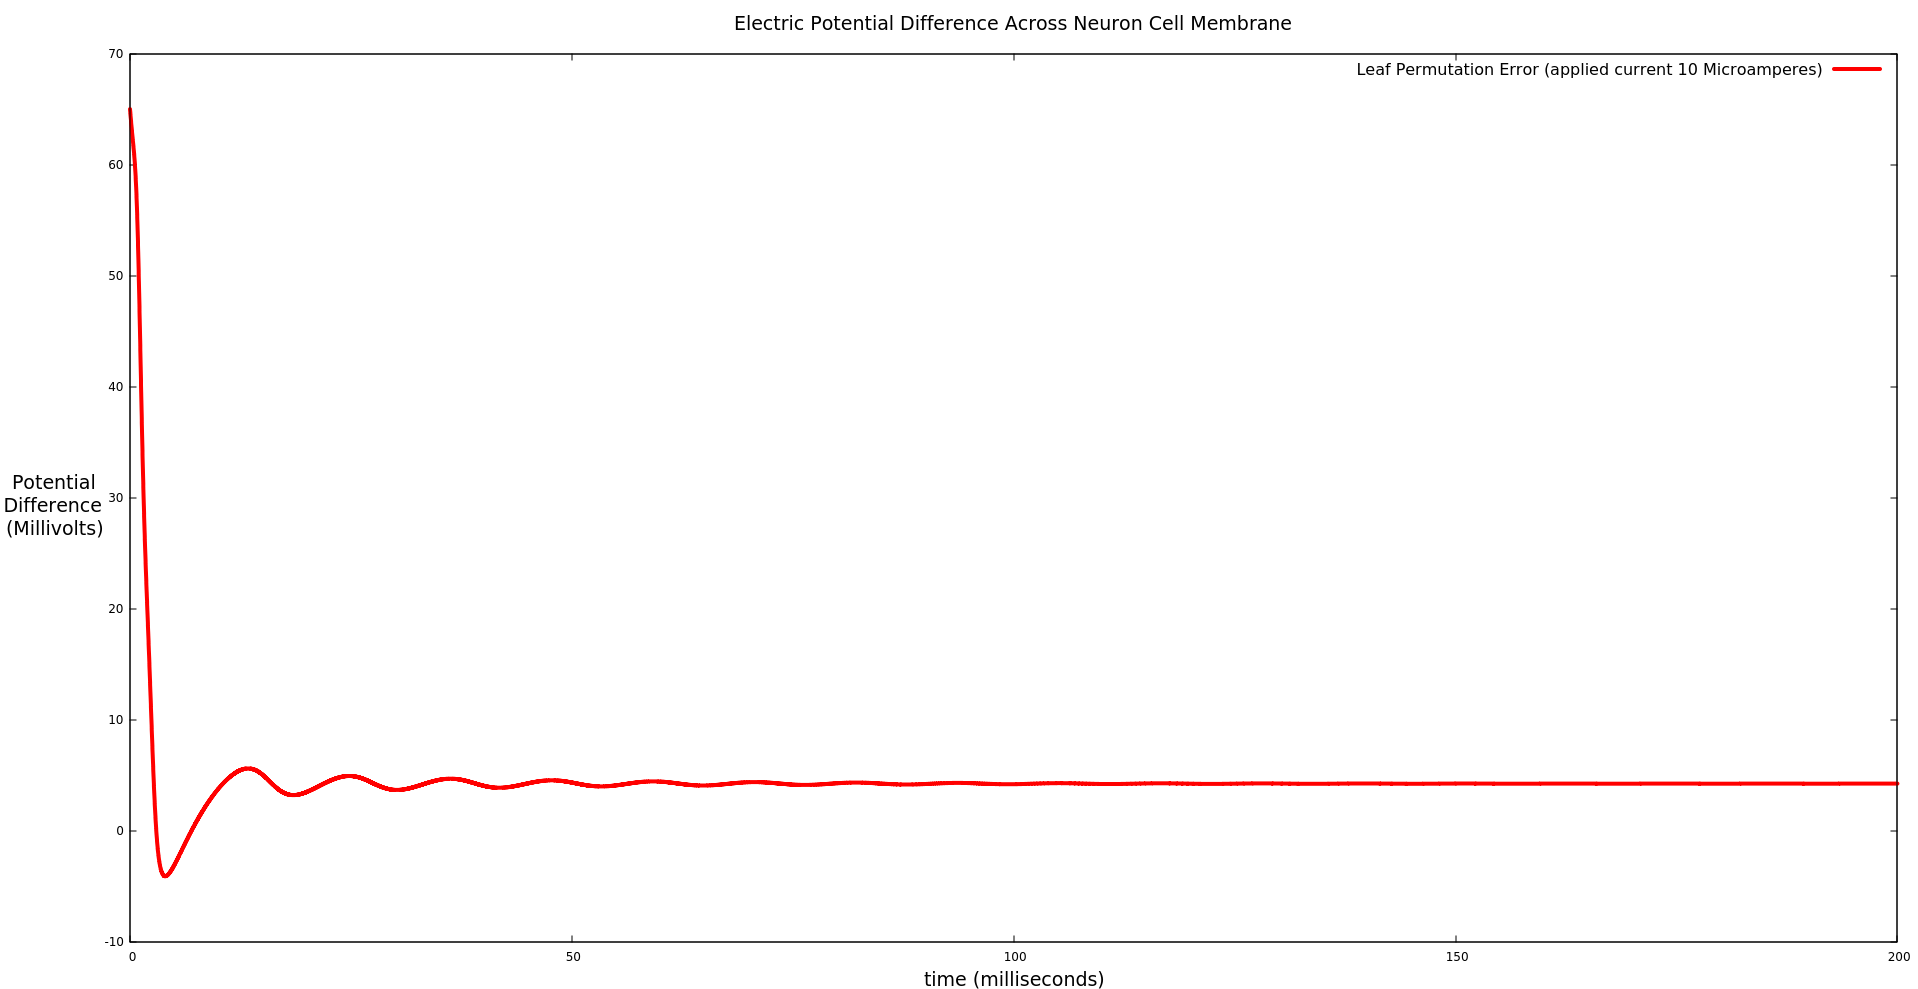
\includegraphics[height = \paperheight, 
      width = \paperwidth]{10MicroampereHH_ERROR.png}}
  \begin{frame}[plain]
  \end{frame}
}

{
  \setbeamertemplate{navigation symbols}{}
  \setbeamertemplate{background canvas}{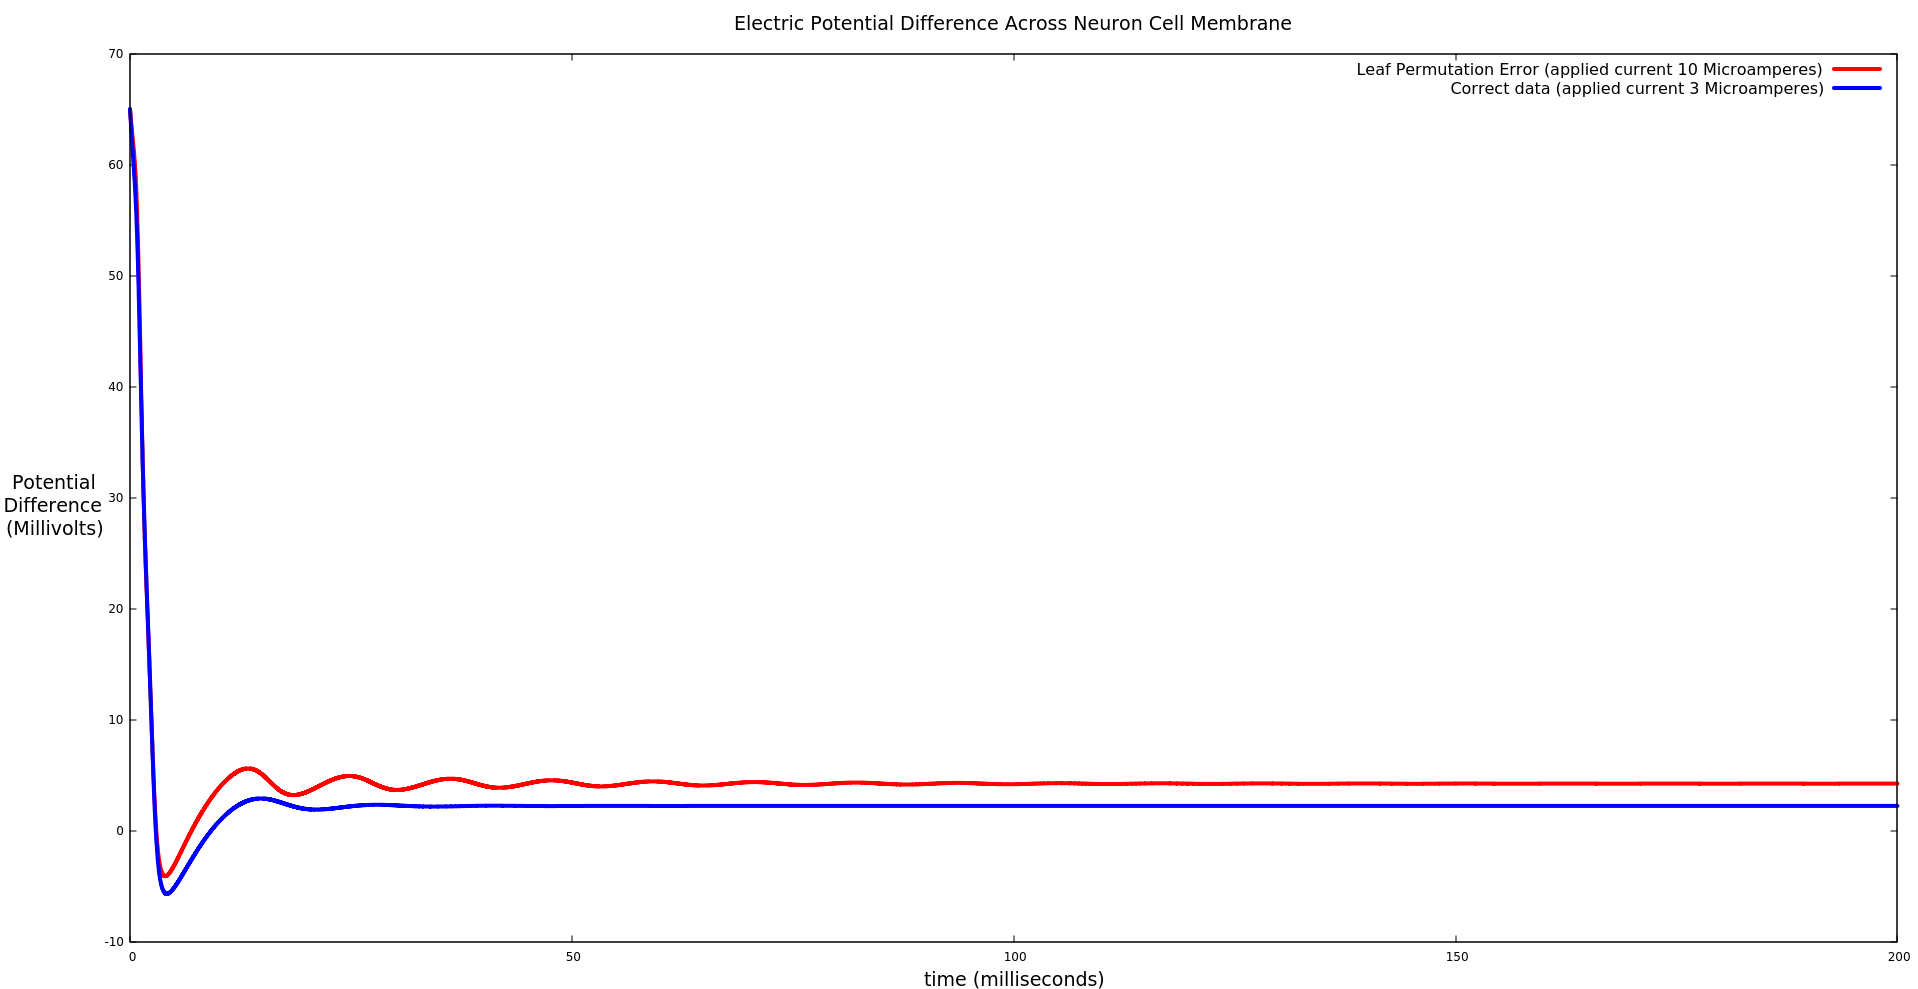
\includegraphics[height = \paperheight, 
      width = \paperwidth]{ErrorComparison.png}}
  \begin{frame}[plain]
  \end{frame}
}

%\begin{frame}[fragile]
%  \begin{minted}{C++}
%  template <typename R, int m, int kg, int s,
%            int K, int A, int mol, int cd>
%
%  Quantity<R, m, kg, s, K, A, mol, cd>
%  operator+(Quantity<R, m, kg, s, K, A, mol, cd> op1,
%            Quantity<R, m, kg, s, K, A, mol, cd> op2)
%  {
%    return Quantity<R, m, kg, s, K, A, mol, cd>{
%      op1.value + op2.value
%    };
%  }  
%  \end{minted}
%
%  \blfootnote{cppsci}
%\end{frame}

\begin{frame}[fragile]
  \begin{minted}{C++}
    Ampere const I     =  10.0;  // micro
    Farad const C      =  1.0;   // micro
    Siemens const g_Na =  120.0; // milli
    Siemens const g_K  =  36.0;  // milli
    Siemens const g_L  =  0.3;   // milli
    Volt const E_Na    =  120.0; // milli
    Volt const E_K     = -12.0;  // milli
    Volt const E_L     =  10.6;  // milli
    
    QuotientType<Volt, second>::type
    dV_wrt_dt(Volt V, dimless n, dimless m, dimless h)
    {
      return (I - g_K*unit_aux::pow4(n)*(V - E_K)
                - g_Na*unit_aux::pow3(m)*h*(V - E_Na)
                - g_L*(V - E_L))
                / C;
    }
  \end{minted}
\end{frame}

\begin{frame}[fragile]
  \begin{forest}
    [/, s sep=10mm, for tree=draw
      [$-$, s sep=12mm, for tree=draw
        [I]
        [*
          [$g_K$]
          [pow [n] [4]]
          [$-$ [V] [$E_K$]]  
        ]
        [*
          [$g_{Na}$]
          [pow [m] [3]]
          [h]
          [$-$ [V] [$E_{Na}$]]
        ]
        [*
          [$g_L$]
          [$-$ [V] [$E_L$]]
        ]
      ]
      [C]
    ]
  \end{forest}
\end{frame}

\begin{frame}[fragile]
  \begin{forest}
    [/, s sep=10mm, for tree=draw
      [$-$, s sep=12mm, for tree=draw
        [I]
        [*
          [$g_K$]
          [pow [n] [4]]
          [$-$ [V] [$E_K$]]  
        ]
        [*
          [$g_{Na}$]
          [pow [m,name=obj2] [3]]
          [h]
          [$-$ [V] [$E_{Na}$]]
        ]
        [*
          [$g_L$]
          [$-$ [V] [$E_L$,name=obj1]
          ]
        ]
      ]
      [C]
    ]
    \draw[->, red] (obj2) to[out=south west, in=south] (obj1);
  \end{forest}
\end{frame}

\begin{frame}[fragile]
  \begin{forest}
    [/, s sep=10mm, for tree=draw
      [$-$, s sep=12mm, for tree=draw
        [I]
        [*
          [$g_K$]
          [pow [n] [4]]
          [$-$ [V] [$E_K$]]  
        ]
        [*
          [$g_{Na}$]
          [pow [$m$,name=obj2] [3]]
          [h]
          [$-$ [V] [$E_{Na}$]]
        ]
        [*
          [$g_L$]
          [$-$ [V] [$m$,name=obj1]
          ]
        ]
      ]
      [C]
    ]
    \draw[->, red] (obj2) to[out=south west, in=south] (obj1);
  \end{forest}

  \pause
  \dots produces a compile time error!!

  \vspace{2mm}

  This program cannot be created, so there are no erroneous results!
\end{frame}

\begin{frame}[fragile]
  \begin{verbatim}
    . . . no match for ‘operator-’
    (operand types are
    ‘unit::Volt
    {aka unit::Quantity<double, 2, 1, -3, 0, -1, 0, 0>}’
    and ‘unit::dimensionless
    {aka unit::Quantity<double, 0, 0, 0, 0, 0, 0, 0>}’)

    return (I - g_K*pow4(n)*(V - E_K)
              - g_Na*pow3(m)*h*(V - E_Na)
              - g_L*(V - m)) / C;
                     ~~^~~
   \end{verbatim}
\end{frame}

\begin{frame}[fragile]
  The number of type-checking leaf permutations $N$ can be found via

  \begin{equation*}
  N = \prod_{leaves} \: n_{leaf}
  \end{equation*}

  where $n_{leaf}$ is the number of in-scope variables that share the same type as the current
  leaf.

  \vspace{2mm}
  \pause
  
  The number of leaf permutations for the program without unit analysis:
  \begin{align*}
    12 & \cdot 12 \cdot \dots \cdot 12 = 12^{14} = 1283918464548864 \\
    \approx & \: 1.28 \times 10^{15}
  \end{align*}

  \pause 

  The number of leaf permutations for the program with unit analysis:
  \begin{align*}
    1^1 & \cdot 3^6 \cdot 4^6 \cdot 1^1 = 2985984 \\
    \approx & \: 2.99 \times 10^6
  \end{align*}
\end{frame}


\end{document}
